
\newpage
\section{Conjuntos Convexos}

\begin{itemize}
	\item Los conjuntos convexos se presentan en diversos contextos de la teoría microeconómica. 
	\bigskip 
	\item En el contexto de la optimización, los conjuntos convexos juegan un rol fundamental para entender cómo plantear y resolver un problema de optimización. 
	\bigskip 
	\item Referencias: Jehle \& Reny, Advanced Microeconomic Theory, capítulo Convex Sets (Appendix), Apunte Optimización capítulo Conjuntos Convexos. 
\end{itemize}


\begin{definicion}
	\textbf{(Conjunto convexos)}
	Sea $S \subseteq \R^n$, $S \neq \phi$. Se dice que $S$ es \textbf{convexo} si: 
	$$\lambda x + ( 1 - \lambda) y \in S ,\quad  \forall x, y \in S , \forall \lambda \in [0,1] $$
\end{definicion}
 
\begin{center}
	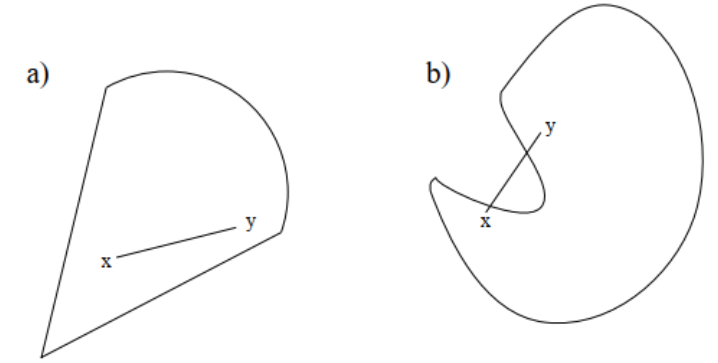
\includegraphics[scale=0.4]{figuras/capitulo2/1.conjuntos-convexos/ej-convexo.png}
\end{center}

	
\begin{itemize}
	\item El conjunto de la figura a) es convexo.  
	\item El conjunto de la figura b) no lo es.  
	\item Un espacio vectorial es un conjunto convexo.  
\end{itemize}

\begin{ejercicio}
	Muestre que $S = \{ x \in \R^3 : x_1 + 2 x_2 - x_3 = 2 \}$ es un conjunto convexo.
	
	\begin{itemize}
		\item Sean $x,y \in S, \lambda \in [0,1]$. Por definición de $S$: 
		$$ x_1 + 2 x_2 - x_3 = 2 $$ 
		$$ y_1 + 2 y_2 - y_3 = 2 $$  
		Por su parte: 
		$$ \lambda x + ( 1 - \lambda ) y = \begin{pmatrix}
			\lambda x_1 +  ( 1- \lambda) y_1 \\
			\lambda x_2 +  ( 1- \lambda) y_2\\
			\lambda x_3 +  ( 1- \lambda) y_3
		\end{pmatrix} $$  
		Y como:
		\begin{eqnarray*}
			& & \lambda x_1 +  ( 1- \lambda) y_1  + 2 (	\lambda x_2 +  ( 1- \lambda) y_2) -(\lambda x_3 +  ( 1- \lambda) y_3)  \\  
			&=& \lambda (x_1 + 2 x_2 - x_3) + (1 - \lambda) (y_1 + 2 y_2 - y_3) \\  
			&=& 2 \lambda + 2( 1 - \lambda ) \\  
			&=& 2 
		\end{eqnarray*} 
		Se concluye que $\lambda x + ( 1 - \lambda ) y \in S$ y, por lo tanto, que $S$ es convexo. $\qed$ 
	\end{itemize} 
\end{ejercicio}


\begin{definicion}
	\textbf{(Hiperplano y semiespacio)}
	Sean $a \in \R^n$ y $\alpha \in \R$ fijos. Se llama \textbf{hiperplano} al conjunto: 
	$$ H = \{ x \in \R^n : a^T x = \alpha \} $$ 
	Un hiperplano $H$ define dos \textbf{semiespacios}: 
	$$ H^- = \{ x \in \R^n : a^T x \leq \alpha \} $$ 
	$$ H ^+  = \{ x \in \R^n : a^T x \geq \alpha \} $$ 
\end{definicion}


\begin{proposicion}
	Un semiespacio $S \in \R^n$ es un conjunto convexo.  
\end{proposicion} 

\begin{proof}
	Consideremos $a \in \R^n$ y $a \in \R$, que definen el semiespacio: 
	$$ S = H^- = \{ x \in \R^n : a^T x \leq \alpha \} $$  
	Sean $x, y \in S$, $\lambda \in [0,1]$, entonces: 
	$$ \alpha ^T [ \lambda x + ( 1 - \lambda ) y ] = \lambda a^T x + ( 1 - \lambda) a ^T y \leq \lambda \alpha + ( 1 - \lambda ) \alpha = \alpha $$  
	Luego, $\lambda x + (1 - \lambda) y \in S$ y, por lo tanto, $S$ es convexo. 
	
	La demostración para $H^+$ es análoga. 
\end{proof}

  


\begin{proposicion}
	Sean $S_1$ y $S_2$ conjuntos convexos. Entonces $S_1 \cap S_2$ es un conjunto convexo. 
\end{proposicion}

\begin{proof}
	Sean $x,y \in S_1 \cap S_2, \lambda \in [0,1]$. Entonces: 
	$$ x, y \in S_1 \Longrightarrow \lambda x + (1 - \lambda) y \in S_1$$ 
	$$ x, y \in S_2 \Longrightarrow \lambda x + (1 - \lambda) y \in S_2 $$
	Gracias a que $S_1$ y $S_2$ son convexos.  
	
	Luego, $\lambda x + ( 1 - \lambda ) y  \in S_1 \cap S_2$ y, por lo tanto, $S_1 \cap S_2$ es convexo.
\end{proof}  


\textbf{Discusión:}
\begin{itemize}
	\item Claramente, la propiedad anterior se puede generalizar a una intersección cualquiera de conjuntos convexos. Es decir, si $(S_i)_{i\in I}$ son conjuntos convexos, entonces $\bigcap _{i\in I} S_i$ es un conjunto convexo.  
	\bigskip 
	\item ¿Qué se puede decir sobre la unión de convexos? 
\end{itemize}

\subsubsection{Sistemas de desigualdades lineales}
\begin{ejemplo}
	Consideremos un sistema de la forma: 
	$$ a_{11} x_1 + ... + a_{1n}x_n \leq b_1 $$ 
	$$ \vdots $$ 
	$$ a_{m1} x_1 + ... + a_{mn} x_n \leq b_m $$ 
	Con $a_{ij}, b_i, x_j \in \R, \forall i = 1, ... , m , j = 1 , ... , n$. 
	De forma simplificada, escribimos: 
	$$ A x \leq b $$ 
	Con $A = (a_{ij})$ y $b = (b_i)$. 
	
	Entonces, el conjunto $S$ dado por: 
	$$ S  = \{ x \in \R^n : A x \leq b \} $$ 
	Es un conjunto convexo. 
\end{ejemplo}

\begin{definicion}
	\textbf{(Combinación convexa)} 
	Sean $x_1, ... , x_k \in \R^n, \lambda_1 , ... \lambda_k \in \R_+$ tales que $\sum_{i = 1}^{k} \lambda_i = 1$. El vector
	$$ x = \sum_{i=1}^{k}\lambda_i x_i $$
	se dice \textbf{combinación convexa} de los $k$ vectores $x_1, ... , x_k$. 
\end{definicion}

\begin{definicion}
	\textbf{(Envoltura convexa)}
	Dado $S\subseteq \R^n$, se define la \textbf{envoltura convexa} de $S$, de la manera siguiente: 
	$$ co (S) = \{ \sum_{i=1}^{k}\lambda_i x_i : k \in \N, x_1, ... , x_k \in S, \lambda_1, ... , \lambda_k \in \R_+ , \sum_{i=1}^{k}\lambda_i = 1 \} $$
	Es decir, el conjunto de todas las posibles combinaciones convexas de puntos de $S$. 
\end{definicion}


\begin{nota}
	\begin{itemize}
		\item $S \subseteq co(S)$  
		\item $S$ es convexos si y solo si $co(S) = S$  
		\item Si $S \subseteq S'$, entonces $co(S) \subseteq co(S')$
	\end{itemize}
\end{nota}

\begin{center}
	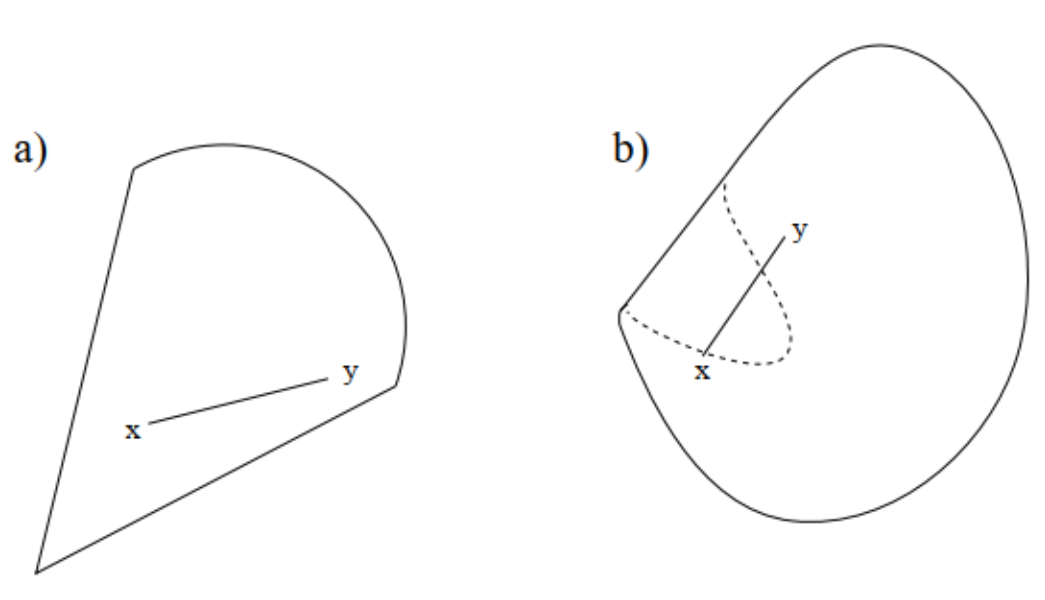
\includegraphics[scale=0.4]{figuras/capitulo2/1.conjuntos-convexos/ej-envoltura-convexa.png}
\end{center}


\begin{itemize}
	\item En la figura a) la envoltura convexa del conjunto es igual a él, pues es convexo. 
	\item En la figura b), la línea sólida corresponde a la envoltura convexa (que contiene al conjunto original).
\end{itemize}


\begin{proposicion}
	Sea $S \subseteq \R^k$. El conjunto $co(S)$ es convexo. 
\end{proposicion}

\begin{proof}
	Sean $x,y \in co(S)$, es decir: 
	$$ x = \sum_{i=1}^n \nu_i x_i , \quad y = \sum_{i=1}^m \mu_i y_i $$
	donde $x_1, ... , x_n, y_1, ... y_m \in S$ y $\nu_1, ... \nu_n, \mu_1, ... , \mu_m$ son ponderadores de las combinaciones convexas.  
	
	Sea $\lambda \in [0,1]$.   
	
	Luego: 
	$$\lambda x + (1 - \lambda)y = \lambda \sum_{i=1}^n  \nu_i x_i + (1 - \lambda) \sum_{i=1}^m \mu_i y_i $$  
	Llamando $z_i = x_i$, $\alpha_i = \lambda \nu_i$ y $z_{n+i} = y_i , \alpha_{n+i} = (1-\lambda)\mu_i$ se tiene que $\lambda x + ( 1 - \lambda) y = \sum_{i=1}^{n+m} \alpha _i z_i $, con: 
	$$ z_i \in S, \alpha_i \in [0,1], \sum_{i=1}^{n+m} \alpha_i = 1 $$  
	Por definición se tiene que $\lambda x + ( 1 - \lambda ) y \in co (S)$ y, por lo tanto, se concluye que $co(S)$ es convexo.  
\end{proof}


\begin{proposicion}
	El conjunto $co(S)$ es el convexo más pequeño (en el sentido de la inclusión) que contiene a $S$, es decir: 
	$$ co(S) = \bigcap \{ C \subseteq \R^n : C \text{  convexo }, S \subseteq C\} $$
\end{proposicion}

\begin{proof}
	Sea $x \in  \bigcap \{ C \subseteq \R^n : C \text{  convexo }, S \subseteq C\}$.   
	
	Entonces, $x \in C, \forall C $ convexo tal que $S \subseteq C$.   
	
	Luego, $x \in co(S)$, que es un convexo particular que contiene a $S$.  
	
	Sean ahora $x \in co(S) $ y $C$ un convexo cualquiera que contiene a $S$.   
	
	Entonces $co (S) \subseteq co (C) = C$, y por lo tanto $x \in C$.   
	
	Luego, $x \in  \bigcap \{ C \subseteq \R^n : C \text{  convexo }, S \subseteq \}$.   
\end{proof}

\begin{proposicion}
	Sean $S_1$ y $S_2$ conjuntos convexos y $\alpha \in \R$. Definimos la suma y ponderación de conjuntos como sigue: 
	$$ S_1 + S_2 = \{ x + y : x \in S_1, y \in S_2 \} $$ 
	$$ \alpha S_1 = \{ \alpha x : x \in S_1 \} $$  
	Se tiene que $S_1 + S_2$ y $\alpha S_1$ son conjuntos convexos. 
\end{proposicion}


\begin{proof}
	\textcolor{red}{To be added...}
\end{proof}